\chapter{Continuous-Time Diffusion and SDEs}
\label{ch:sde}

Generative modeling via diffusion processes has revolutionized artificial intelligence, establishing new state-of-the-art results across image, audio, and structural generation. In the preceding chapters, we explored score-based generative modeling and Denoising Diffusion Probabilistic Models (DDPMs) through the lens of discrete Markov chains. While the discrete-time formulation provides an intuitive framework for implementation, it introduces arbitrary discretization artifacts and obscures the elegant geometrical and topological properties of the underlying dynamics. When the number of diffusion steps approaches infinity and the step size vanishes to zero, the discrete Markov chains of DDPM converge to continuous-time stochastic processes.

In this chapter, we elevate the diffusion framework to continuous time using Stochastic Differential Equations (SDEs). By taking the limit of infinite time steps, the forward corruption process and the reverse generation process both converge to paths governed by SDEs. This continuous-time perspective, pioneered by Song et al. (2021), offers several profound advantages over its discrete counterpart. First, it unifies previously disparate discrete methods---such as Score Matching with Langevin Dynamics (SMLD) and DDPMs---under a single mathematical umbrella. Different discrete diffusion models are simply different discretization schemes of different continuous-time SDEs. 

Second, the continuous-time framework enables the use of off-the-shelf, black-box ODE and SDE solvers for generation. By separating the mathematical definition of the model from the numerical algorithm used to sample from it, practitioners can seamlessly trade off between generation speed and sample quality without retraining the neural network. This decoupling has led to the development of highly efficient samplers that can generate high-fidelity images in just a handful of steps.

Finally, and perhaps most elegantly, the SDE formalism reveals the existence of the Probability Flow Ordinary Differential Equation (ODE). This is a strictly deterministic process whose trajectories share the exact same marginal probability densities as the stochastic reverse process. The Probability Flow ODE effectively transforms the diffusion model into a continuous normalizing flow, unlocking the ability to compute exact data log-likelihoods and seamlessly manipulate latent representations.

At its core, a continuous-time diffusion model defines a forward SDE that smoothly morphs a complex, empirical data distribution into a tractable prior distribution (such as a standard isotropic Gaussian). The information about the original data distribution is gradually annihilated by the continuous injection of Brownian noise. The magic of the SDE framework, rooted in the foundational theorems of stochastic calculus, is that this information destruction is perfectly reversible. If we know the score of the marginal distributions at every point in time---that is, the gradient of the log probability density with respect to the data---we can construct a reverse-time SDE that starts from the noise prior and flawlessly reconstructs the original data distribution. The training of a continuous-time diffusion model therefore reduces to score matching: training a neural network to estimate these continuous-time scores.

We will begin our exploration by defining the mathematical machinery of SDEs and the Fokker-Planck equation, which governs the evolution of probability densities. We then proceed to Anderson's theorem, which guarantees the existence of the reverse SDE. Building upon these foundations, we derive the continuous-time score matching objective and the celebrated Probability Flow ODE, concluding with a numerical example of the Variance Preserving (VP) SDE.


\section{The Forward Stochastic Differential Equation}

Let $x \in \mathbb{R}^d$ denote a continuous random variable. We consider a continuous-time parameter $t \in [0, T]$, where $t=0$ corresponds to the data distribution and $t=T$ corresponds to the noise prior. Following our established notation, the data distribution is denoted as $p_0(x) \equiv P_{\text{data}}(x)$.

A continuous-time diffusion process $\{x(t)\}_{t \in [0, T]}$ is governed by the following It\^{o} SDE:
\begin{equation}
\label{eq:forward_sde}
dx = f(x, t) dt + g(t) dw
\end{equation}
where $f(x, t) \in \mathbb{R}^d$ is the drift coefficient (a deterministic vector field), $g(t) \in \mathbb{R}$ is the diffusion coefficient (a scalar function), and $w(t) \in \mathbb{R}^d$ is a standard Brownian motion (or Wiener process). 

The marginal probability density of the process at time $t$ is denoted by $p_t(x)$. As the process evolves from $t=0$ to $t=T$, the data distribution $p_0(x)$ is transformed into the prior distribution $p_T(x)$, which we typically design to be an unstructured distribution that contains no information about $p_0(x)$, such as $\mathcal{N}(0, I)$.

The evolution of the marginal density $p_t(x)$ over time is exactly described by the Fokker-Planck equation (also known as the Kolmogorov forward equation).

\begin{theorem}[Fokker-Planck Equation]
\label{thm:fokker_planck}
Let $x(t)$ be the solution to the SDE in Equation~\ref{eq:forward_sde}. The marginal probability density function $p_t(x)$ satisfies the partial differential equation:
\begin{equation}
\frac{\partial p_t(x)}{\partial t} = -\nabla_x \cdot (f(x, t) p_t(x)) + \frac{1}{2} g(t)^2 \Delta_x p_t(x)
\end{equation}
where $\nabla_x \cdot$ denotes the divergence operator and $\Delta_x = \nabla_x \cdot \nabla_x$ is the Laplacian.
\end{theorem}
The proof of Theorem~\ref{thm:fokker_planck} follows from It\^{o}'s Lemma and integration by parts against smooth test functions, representing the conservation of probability mass under the advection-diffusion dynamics.


\section{The Reverse Stochastic Differential Equation}

The most remarkable result in the theory of diffusion models is that the forward process can be rigorously reversed. Anderson (1982) demonstrated that for every forward SDE, there exists a corresponding reverse-time SDE that traverses the exact same marginal distributions in reverse, from $t=T$ down to $t=0$.

\begin{theorem}[Anderson's Reverse SDE]
\label{thm:reverse_sde}
The reverse-time process corresponding to the forward SDE $dx = f(x, t) dt + g(t) dw$ is given by the SDE:
\begin{equation}
\label{eq:reverse_sde}
d\bar{x} = \left[ f(\bar{x}, t) - g(t)^2 \nabla_{\bar{x}} \log p_t(\bar{x}) \right] dt + g(t) d\bar{w}
\end{equation}
where $dt$ is a negative, infinitesimal time step (time flows backwards from $T$ to $0$), and $\bar{w}$ is a standard Brownian motion when time is reversed.
\end{theorem}

\begin{proof}
We derive this by equating the Fokker-Planck equations of the forward and reverse processes. Let the reverse process be parameterized as $d\bar{x} = \tilde{f}(\bar{x}, t) dt + g(t) d\bar{w}$. Note that the diffusion coefficient $g(t)$ must remain the same for the stochastic volatility of the paths to match. 

Since time runs backwards in the reverse SDE, the Fokker-Planck equation for the reverse process dictates the change in density as $t$ decreases. Let $\tau = T - t$ represent forward time in the reverse process. The standard Fokker-Planck equation in $\tau$ is:
\begin{equation}
\frac{\partial p_{T-\tau}(x)}{\partial \tau} = -\nabla_x \cdot (\tilde{f}(x, T-\tau) p_{T-\tau}(x)) + \frac{1}{2} g(T-\tau)^2 \Delta_x p_{T-\tau}(x)
\end{equation}
Using the chain rule, $\frac{\partial p_t}{\partial \tau} = \frac{\partial p_t}{\partial t} \frac{dt}{d\tau} = -\frac{\partial p_t}{\partial t}$. Thus, in terms of $t$, the reverse Fokker-Planck equation is:
\begin{equation}
-\frac{\partial p_t(x)}{\partial t} = -\nabla_x \cdot (\tilde{f}(x, t) p_t(x)) + \frac{1}{2} g(t)^2 \Delta_x p_t(x)
\end{equation}
Substitute the forward Fokker-Planck equation (Theorem~\ref{thm:fokker_planck}) into the left-hand side:
\begin{equation}
\nabla_x \cdot (f(x, t) p_t(x)) - \frac{1}{2} g(t)^2 \Delta_x p_t(x) = -\nabla_x \cdot (\tilde{f}(x, t) p_t(x)) + \frac{1}{2} g(t)^2 \Delta_x p_t(x)
\end{equation}
Rearranging the terms to group divergences, we obtain:
\begin{equation}
\nabla_x \cdot \left[ (f(x, t) + \tilde{f}(x, t)) p_t(x) \right] = g(t)^2 \Delta_x p_t(x)
\end{equation}
Using the fundamental identity $\Delta_x p_t(x) = \nabla_x \cdot (\nabla_x p_t(x)) = \nabla_x \cdot (p_t(x) \nabla_x \log p_t(x))$, we have:
\begin{equation}
\nabla_x \cdot \left[ (f(x, t) + \tilde{f}(x, t)) p_t(x) \right] = \nabla_x \cdot \left[ g(t)^2 p_t(x) \nabla_x \log p_t(x) \right]
\end{equation}
A sufficient condition for this equality to hold uniformly over $x$ is:
\begin{equation}
(f(x, t) + \tilde{f}(x, t)) p_t(x) = g(t)^2 p_t(x) \nabla_x \log p_t(x)
\end{equation}
Dividing by $p_t(x)$ and solving for the reverse drift $\tilde{f}(x, t)$, we find:
\begin{equation}
\tilde{f}(x, t) = -f(x, t) + g(t)^2 \nabla_x \log p_t(x)
\end{equation}
In the simulation of the reverse SDE, the time differential $dt$ is strictly negative. The effective drift vector we follow is:
\begin{equation}
dx = -\tilde{f}(x, t) |dt| + g(t) d\bar{w} = \left[ f(x, t) - g(t)^2 \nabla_x \log p_t(x) \right] dt + g(t) d\bar{w}
\end{equation}
which concludes the proof.
\end{proof}

\begin{figure}[ht]
\centering
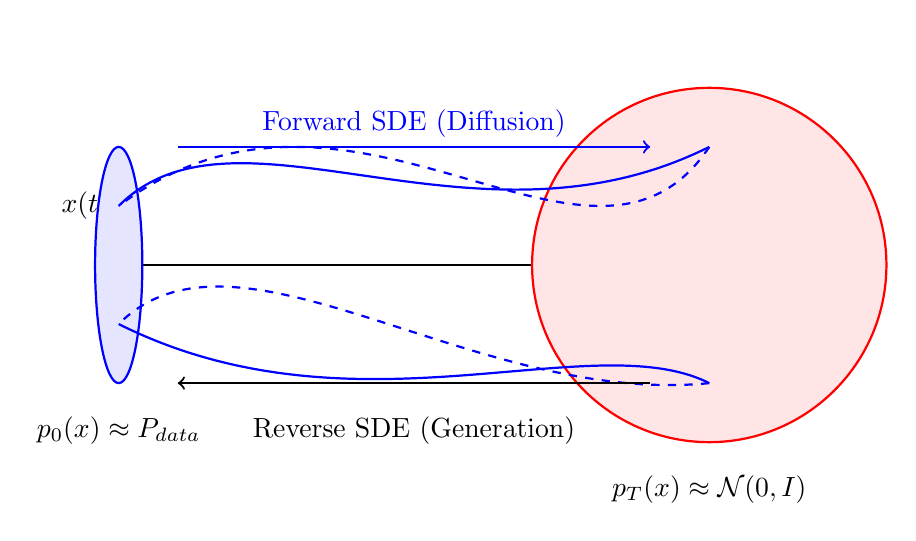
\begin{tikzpicture}[scale=1.5]
  % Forward process
  \draw[->, thick] (0, 0) -- (5, 0) node[right] {$t$};
  \node[left] at (0, 0.5) {$x(t)$};
  
  % Initial distribution (Data)
  \draw[thick, blue, fill=blue!10] (0, 0) ellipse [x radius=0.2, y radius=1];
  \node[below] at (0, -1.2) {$p_0(x) \approx P_{\text{data}}$};
  
  % Final distribution (Noise)
  \draw[thick, red, fill=red!10] (5, 0) circle [radius=1.5];
  \node[below] at (5, -1.7) {$p_T(x) \approx \mathcal{N}(0, I)$};

  % Forward trajectory 1
  \draw[blue, thick] (0, 0.5) .. controls (1, 1.5) and (3, 0) .. (5, 1);
  \draw[blue, thick, dashed] (5, 1) .. controls (4, -0.5) and (2, 2) .. (0, 0.5);

  % Forward trajectory 2
  \draw[blue, thick] (0, -0.5) .. controls (2, -1.5) and (4, -0.5) .. (5, -1);
  \draw[blue, thick, dashed] (5, -1) .. controls (3, -1.2) and (1, 0.5) .. (0, -0.5);

  \node[blue, above] at (2.5, 1) {Forward SDE (Diffusion)};
  \node[black, below] at (2.5, -1.2) {Reverse SDE (Generation)};
  \draw[<-, thick, black] (0.5, -1) -- (4.5, -1);
  \draw[->, thick, blue] (0.5, 1) -- (4.5, 1);

\end{tikzpicture}
\caption{Schematic representation of continuous-time diffusion. The forward SDE diffuses the complex data distribution into an isotropic Gaussian. The reverse SDE deterministically tracks the exact same sequence of marginals in reverse.}
\label{fig:sde_diagram}
\end{figure}


\section{Continuous-Time Score Matching}

To simulate the reverse SDE and generate data, we must know the Stein score function $\nabla_x \log p_t(x)$ for all $t \in [0, T]$. As the true marginal density $p_t(x)$ is generally intractable, we parameterize a neural network $s_\theta(x, t)$ to approximate it.

The objective is to minimize the expected Fisher divergence between the true score and our parameterized score over all times $t$, weighted by a positive function $\lambda(t)$:
\begin{equation}
\mathcal{L}(\theta) = \mathbb{E}_{t \sim \mathcal{U}[0,T]} \left[ \lambda(t) \mathbb{E}_{x(0) \sim p_0} \mathbb{E}_{x(t) \sim p_{t|0}(x(t)|x(0))} \left[ \left\lVert s_\theta(x(t), t) - \nabla_{x(t)} \log p_{t|0}(x(t) | x(0)) \right\rVert_2^2 \right] \right]
\end{equation}
This is the continuous-time equivalent of Denoising Score Matching. Because the forward process is often chosen to be an affine Gaussian (such as a Variance Preserving or Variance Exploding SDE), the transition probability $p_{t|0}(x(t) | x(0))$ is available in closed form, typically $\mathcal{N}(x(t); \mu_t x(0), \sigma_t^2 I)$. Consequently, $\nabla_{x(t)} \log p_{t|0}(x(t) | x(0))$ is analytically trivial to compute as $-(x(t) - \mu_t x(0)) / \sigma_t^2$.


\section{The Probability Flow ODE}

While the reverse SDE provides a mathematically rigorous generative model, it injects noise and thus explores a stochastic path back to the data manifold. A fascinating corollary of the Fokker-Planck equation is that there exists a deterministic differential equation that possesses identical marginals.

\begin{theorem}[Probability Flow ODE]
\label{thm:prob_flow}
The deterministic ordinary differential equation:
\begin{equation}
\label{eq:prob_flow_ode}
dx = \left[ f(x, t) - \frac{1}{2} g(t)^2 \nabla_x \log p_t(x) \right] dt
\end{equation}
has the same marginal probability densities $p_t(x)$ as the forward SDE (Equation~\ref{eq:forward_sde}) for all $t \in [0, T]$.
\end{theorem}
\begin{proof}
Let us find the Fokker-Planck equation for an ODE with drift $F(x, t)$ and zero diffusion ($g=0$).
The equation is:
\begin{equation}
\frac{\partial p_t}{\partial t} = -\nabla_x \cdot (F(x, t) p_t(x))
\end{equation}
We want this temporal derivative to exactly match the forward Fokker-Planck equation of our original SDE:
\begin{equation}
-\nabla_x \cdot (F(x, t) p_t(x)) = -\nabla_x \cdot (f(x, t) p_t(x)) + \frac{1}{2} g(t)^2 \Delta_x p_t(x)
\end{equation}
Using the identity $\Delta_x p_t(x) = \nabla_x \cdot (p_t(x) \nabla_x \log p_t(x))$ again, we rewrite the RHS:
\begin{equation}
-\nabla_x \cdot (F(x, t) p_t(x)) = -\nabla_x \cdot \left( f(x, t) p_t(x) - \frac{1}{2} g(t)^2 p_t(x) \nabla_x \log p_t(x) \right)
\end{equation}
Equating the terms inside the divergence operator yields:
\begin{equation}
F(x, t) p_t(x) = f(x, t) p_t(x) - \frac{1}{2} g(t)^2 p_t(x) \nabla_x \log p_t(x)
\end{equation}
Dividing by $p_t(x)$, we arrive at the drift for our deterministic ODE:
\begin{equation}
F(x, t) = f(x, t) - \frac{1}{2} g(t)^2 \nabla_x \log p_t(x)
\end{equation}
Thus, the ODE defined by $dx = F(x, t)dt$ correctly marginalizes to $p_t(x)$ at every instant $t$.
\end{proof}

The Probability Flow ODE acts as a deterministic map between the latent space and the data space. This means continuous-time diffusion models can be rigorously formulated as continuous normalizing flows, allowing us to compute exact log-likelihoods via the instantaneous change of variables formula.

\begin{figure}[ht]
\centering
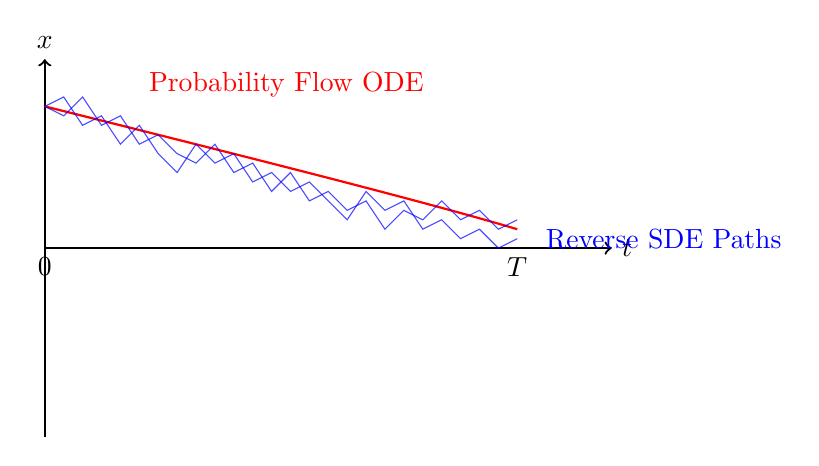
\begin{tikzpicture}[scale=1.2]
  % Axes
  \draw[->, thick] (0, 0) -- (6, 0) node[right] {$t$};
  \draw[->, thick] (0, -2) -- (0, 2) node[above] {$x$};
  
  \node[below] at (0, 0) {$0$};
  \node[below] at (5, 0) {$T$};
  
  % Trajectories
  % True ODE trajectory
  \draw[red, thick] (0, 1.5) .. controls (2, 1.0) and (4, 0.5) .. (5, 0.2);
  
  % SDE trajectories
  \draw[blue, thin, opacity=0.7] (0, 1.5) -- (0.2, 1.6) -- (0.4, 1.3) -- (0.6, 1.4) -- (0.8, 1.1) -- (1.0, 1.3) -- (1.2, 1.0) -- (1.4, 0.8) -- (1.6, 1.1) -- (1.8, 0.9) -- (2.0, 1.0) -- (2.2, 0.7) -- (2.4, 0.8) -- (2.6, 0.6) -- (2.8, 0.7) -- (3.0, 0.5) -- (3.2, 0.3) -- (3.4, 0.6) -- (3.6, 0.4) -- (3.8, 0.5) -- (4.0, 0.2) -- (4.2, 0.3) -- (4.4, 0.1) -- (4.6, 0.2) -- (4.8, 0.0) -- (5.0, 0.1);

  \draw[blue, thin, opacity=0.7] (0, 1.5) -- (0.2, 1.4) -- (0.4, 1.6) -- (0.6, 1.3) -- (0.8, 1.4) -- (1.0, 1.1) -- (1.2, 1.2) -- (1.4, 1.0) -- (1.6, 0.9) -- (1.8, 1.1) -- (2.0, 0.8) -- (2.2, 0.9) -- (2.4, 0.6) -- (2.6, 0.8) -- (2.8, 0.5) -- (3.0, 0.6) -- (3.2, 0.4) -- (3.4, 0.5) -- (3.6, 0.2) -- (3.8, 0.4) -- (4.0, 0.3) -- (4.2, 0.5) -- (4.4, 0.3) -- (4.6, 0.4) -- (4.8, 0.2) -- (5.0, 0.3);
  
  \node[red, above right] at (1, 1.5) {Probability Flow ODE};
  \node[blue, right] at (5.2, 0.1) {Reverse SDE Paths};
\end{tikzpicture}
\caption{A visualization comparing the deterministic trajectories of the Probability Flow ODE with the stochastic paths of the Reverse SDE. Both processes lead to identical marginal probability distributions $p_t(x)$.}
\label{fig:ode_vs_sde}
\end{figure}


\section{Numerical Example: The Variance Preserving (VP) SDE}

Consider the continuous-time generalization of the standard DDPM process, known as the Variance Preserving (VP) SDE. The forward equation is defined as:
\begin{equation}
dx = -\frac{1}{2} \beta(t) x dt + \sqrt{\beta(t)} dw
\end{equation}
where $\beta(t)$ is a continuous, strictly positive noise schedule. This dynamical system is recognized as an Ornstein-Uhlenbeck (OU) process. It exerts a restorative drift force pulling the state toward the origin, counteracting the expanding variance introduced by the Brownian noise.

Given a deterministic starting point $x(0)$, the transition kernel is Gaussian. We can solve this linear SDE explicitly using standard integrating factors. Let $\alpha(t) = \exp\left(-\int_0^t \beta(s) ds\right)$. The transition kernel is:
\begin{equation}
p_{t|0}(x(t) | x(0)) = \mathcal{N}\left(x(t); \sqrt{\alpha(t)} x(0), (1 - \alpha(t)) I \right)
\end{equation}
As $t \to \infty$, if the integral of the noise schedule diverges ($\int_0^\infty \beta(s) ds \to \infty$), then $\alpha(t) \to 0$, and the distribution converges exactly to the standard normal prior $\mathcal{N}(0, I)$.

The corresponding reverse SDE, which we simulate to generate samples, is directly obtained by applying Theorem~\ref{thm:reverse_sde}:
\begin{equation}
d\bar{x} = \left[ -\frac{1}{2} \beta(t) \bar{x} - \beta(t) \nabla_{\bar{x}} \log p_t(\bar{x}) \right] dt + \sqrt{\beta(t)} d\bar{w}
\end{equation}

Similarly, the Probability Flow ODE is:
\begin{equation}
d\bar{x} = -\frac{1}{2} \beta(t) \left[ \bar{x} + \nabla_{\bar{x}} \log p_t(\bar{x}) \right] dt
\end{equation}
By replacing the true score $\nabla_{\bar{x}} \log p_t(\bar{x})$ with our trained neural network approximation $s_\theta(\bar{x}, t)$, we are fully equipped to implement either stochastic or deterministic generative samplers using standard differential equation libraries.


\begin{horizon}
The equivalence between SDEs and ODEs via the Fokker-Planck equation resolves a fundamental theoretical question in continuous-time generative modeling, but leaves open profound computational challenges. It is conjectured that there exists an optimal transport metric under which the probability flow ODE yields geodesics---the geometrically shortest paths of information destruction. If this optimal geometry can be analytically identified and integrated directly into the neural network's architecture, sampling could potentially be achieved in a single, lightning-fast forward pass without any discretization error.

Furthermore, while Anderson's theorem handles forward processes where the diffusion coefficient $g(t)$ is isotropic and data-independent, future work might show that adaptive, state-dependent noise schedules $g(x, t)$ can radically accelerate the mixing time. An open question is whether one can construct a non-linear forward SDE whose spectrum naturally disentangles the semantic factors of variation, mapping high-level generative concepts to the slowest-decaying eigenfunctions of the associated Fokker-Planck operator. 
\end{horizon}


\section{Summary}
\begin{itemize}
    \item Continuous-time diffusion models utilize Stochastic Differential Equations (SDEs) to provide a unified, geometrically rigorous mathematical framework for score-based generative modeling.
    \item The forward SDE steadily diffuses the data distribution into pure noise, with its marginal densities evolving according to the celebrated Fokker-Planck equation.
    \item Anderson's theorem provides a reverse-time SDE capable of exactly reconstructing the original data distribution from noise, provided we know the true score function $\nabla_x \log p_t(x)$.
    \item The Probability Flow ODE is a strictly deterministic counterpart to the reverse SDE that maintains an identical sequence of marginal probability distributions, enabling exact likelihood computation and continuous normalizing flow interpretation.
\end{itemize}

\section{Exercises}
\begin{enumerate}
    \item \textbf{Variance Exploding SDE}: The Variance Exploding (VE) SDE is given by $dx = \sqrt{\frac{d [\sigma^2(t)]}{dt}} dw$ with zero drift. Derive the transition kernel $p_{t|0}(x(t)|x(0))$ and write down the corresponding reverse SDE and Probability Flow ODE.
    \item \textbf{Fokker-Planck for VP-SDE}: Substitute the drift and diffusion coefficients of the VP-SDE into the Fokker-Planck equation. Verify that the stationary distribution is $\mathcal{N}(0, I)$ by setting $\frac{\partial p_t(x)}{\partial t} = 0$.
    \item \textbf{Likelihood Computation}: Using the instantaneous change of variables formula for neural ODEs, write down the integral required to compute the exact log-likelihood $\log p_0(x)$ of a data point using the Probability Flow ODE.
\end{enumerate}

% TODO-CITE: Ensure all named results are cited.
